\documentclass{article}
\usepackage{graphicx} % Required for inserting images
\usepackage[a4paper,margin=2.5cm]{geometry}
\usepackage{amsmath}
\usepackage{float}
\usepackage{xcolor}
\usepackage{listings}
\usepackage{caption}
\usepackage{subcaption}
\usepackage{xparse}
\usepackage{hyperref}
\usepackage{amssymb}
\usepackage{verbatim}
\usepackage{fancyhdr}
\pagestyle{fancy}
\usepackage{xspace}
\cfoot{}
\lfoot{SMOS, Universitat Politècnica de Catalunya, year 2023-24}
\rfoot{\thepage}

\definecolor{codegreen}{rgb}{0,0.6,0}
\definecolor{codegray}{rgb}{0.5,0.5,0.5}
\definecolor{codepurple}{rgb}{0.58,0,0.82}
\definecolor{backcolour}{rgb}{0.95,0.95,0.92}

\lstdefinestyle{mystyle}{
    backgroundcolor=\color{backcolour},   
    commentstyle=\color{codegreen},
    keywordstyle=\color{magenta},
    numberstyle=\tiny\color{codegray},
    stringstyle=\color{codepurple},
    basicstyle=\ttfamily\footnotesize,
    breakatwhitespace=false,         
    breaklines=true,                 
    captionpos=b,                    
    keepspaces=true,                 
    numbers=left,                    
    numbersep=5pt,                  
    showspaces=false,                
    showstringspaces=false,
    showtabs=false,                  
    tabsize=2
}

\lstset{style=mystyle}

\title{\textbf{Central Limit Theorem}}
\author{Student: Giacomo Calabria}
\date{}

\begin{document}

\maketitle

\section*{Introduction}
In this first module we consider the problem of throwing dice multiple times and using and calculating the resulting probability distribution. In this scenario, $N_{dice}$ dice are thrown $N_{iter}$ times.
\section{Figure 1}
We starty by generating $N_{iter}$ random numbers and use them for the calculation of the probability distribution.\\\\
The random variable of interest is
\begin{equation}
    x=\text{rand}(6)
\end{equation}
and the theoretical distribution is uniform and is $p_i=\frac16$.\\\\
We use the following code we generate the random distribution
\begin{lstlisting}[language=Python]
Niter = 1000
dice_rolls = [random.randint(1, 6) for _ in range(Niter)]
counts = [dice_rolls.count(i) for i in range(1, 7)]
pdf = np.array(counts)/Niter
plt.bar(range(1, 7), pdf)
\end{lstlisting}
In line 4 we normalise the counter in order to obtain the probability distribution.\\\\
We generated the distribution for $N_{iter}=10^3$ and $N_{iter}=10^6$ and reported them in \autoref{fig:1}
\begin{figure}[H]
    \centering
    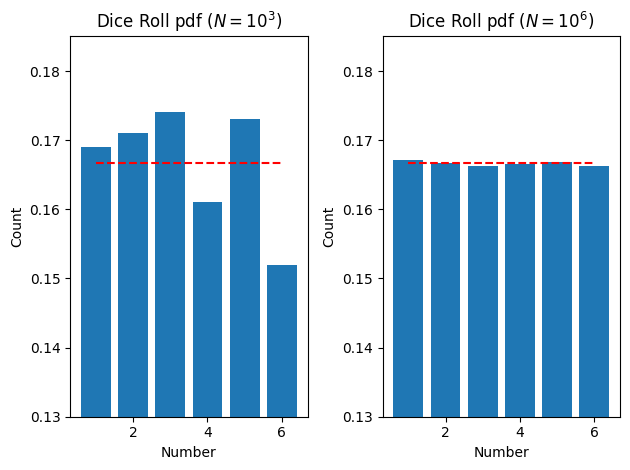
\includegraphics[width=.7\linewidth]{images/Figure1b.png}
    \caption{Simple distribution of dice roll}
    \label{fig:1}
\end{figure}
\noindent As can be seen as the number of $N_{iter}$ iterations increases, the graph tends toward the normal distribution, which was highlighted with the dashed red line.
\clearpage
\section{Figure 2}
We now throw a dice twice, so $N_{dice}=2$ and calculating the average value as
\begin{equation}
    x=\frac{\text{rand}(6)+\text{rand}(6)}2
\end{equation}
We are now going to calculate the the probability distribution of the outcome $x=(1,1.5,2,2.5,\dots,6)$ and plot it into a figure. We use the following code we generate the random distribution
\begin{lstlisting}[language=Python]
Niter = 100000
for i in range(Niter):
    a = random.randint(1, 6)
    b = random.randint(1, 6)
    dice_outcome[i] = (a + b) / 2
bin_edges = np.arange(1, 7, 0.5)
counts, _ = np.histogram(dice_outcome, bins=bin_edges)
pdf = counts / Niter
plt.bar(bin_edges[:-1], pdf, width=0.5)
\end{lstlisting}
\begin{figure}[H]
    \centering
    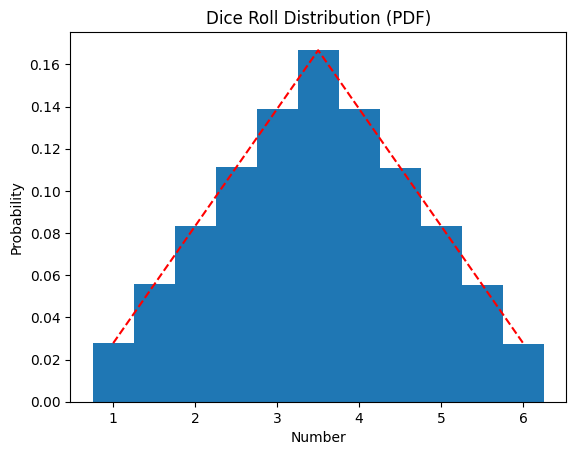
\includegraphics[width=.9\linewidth]{images/Figure2.png}
    \caption{Distribution of the average value of two dice roll}
    \label{fig:2}
\end{figure}
The graph tends toward the normal distribution, which was highlighted with the dashed red line.
\clearpage
\section{Figure 3}
We now consider the follow random event: throwing a dice $N_{iter}$ times and calculating the average value.
\begin{equation}
    x=\frac{\sum_{i=1}^{N_{iter}}{\text{rand}(6)}}{N_{iter}}
\end{equation}
With that random event $x$ we calculate the probability distribution $p(x)$. As we use large $N$ we can consider the random value $x$ as a continuous variable. And then we normalise the PDF as $\int{p(x)dx}=1$.
With this code we generate calculate the probability distribution:
\begin{lstlisting}[language=Python]
Ndice = 100000
Niter = 1000
def random_event():
    return np.sum([random.randint(1, 6) for _ in range(Niter)])/Niter

random_outcome = [random_event() for _ in range(Ndice)]
hist, bins = np.histogram(random_outcome, bins=50, density=True)
bin_centers = (bins[:-1] + bins[1:]) / 2
plt.plot(bin_centers, hist, label='Computed distribution')

x = np.linspace(min(random_outcome)-0.1, max(random_outcome)+0.1, 1000)
gaussian = norm.pdf(x, loc=3.5, scale=np.std(random_outcome))
plt.plot(x, gaussian, label='Gaussian distribution',color='red', linestyle='--')
\end{lstlisting}
\begin{figure}[H]
    \centering
    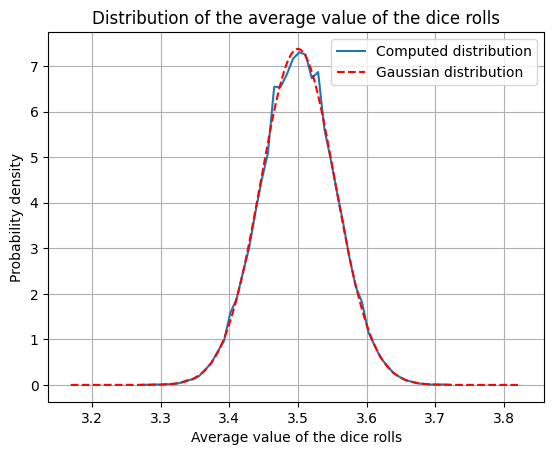
\includegraphics[width=.9\linewidth]{images/Figure3.png}
    \caption{Distribution of the average value of multiple dice roll}
    \label{fig:3}
\end{figure}
As we can see as we use a large number of dice the resulting distribution is pretty similar to the Gaussian distribution expected by the Central Limit Theorem
\clearpage
\section{Error estimation}
We wanna now calculate the average value and estimate the statistical error, associated with such estimation. Assume that single-die throwing is used to estimate the mean value and the variance
\begin{equation}
    \mu=\langle x\rangle\approx\frac{\sum_{i=1}^{N_{iter}}{x_i}}{N_{iter}}
\end{equation}
\begin{equation}
    \sigma^2=\langle x^2\rangle-\langle x \rangle^2\approx\frac{\sum_{i=1}^{N_{iter}}{x_i^2}}{N_{iter}}-\left(\frac{\sum_{i=1}^{N_{iter}}{x_i}}{N_{iter}}\right)^2
\end{equation}
Calculate the mean value by throwing the dice $N_{iter}=10$ and $N_{iter}=100$ times and compare the estimation of the mean value and the variance with the exact values, given by
\begin{equation*}
    \mu=\langle x\rangle=\frac{\sum_{\ell=1}^{6}{\ell}}{6}=3.5\quad \sigma^2=\frac{\sum_{\ell=1}^{6}{\ell^2}}{6}-\left(\frac{\sum_{\ell=1}^{6}{\ell}}{6}\right)^2=\frac{35}{12}\approxeq2.92
\end{equation*}
Using the following code
\begin{lstlisting}[language=Python]
Niter = 10
dice_rolls = np.array([random.randint(1, 6) for _ in range(Niter)])

u = np.sum(dice_rolls)/Niter
var = np.sum(dice_rolls**2)/Niter-np.mean(dice_rolls)**2 # s^2
err = np.sqrt(var/Niter) # (s^2/N)
\end{lstlisting}
then we estimate the statistical error using
\begin{equation}
    \varepsilon=\frac\sigma{\sqrt{N_{iter}}}
\end{equation}
where the variance is the estimation of the statistical error. We obatin the results, which are reported in \autoref{tab:1}
\begin{table}[H]
    \centering
    \begin{tabular}{|l|c|c|c|c|}
        \hline $N_{iter}$  & $\mu$ & $\sigma^2$ &  $\varepsilon $ & $\mu(N_{iter})-\mu_{exact}$\\\hline\hline
        10 & 3.600 & 3.44 & 0.5865 & 0.1\\\hline
        100 & 3.640 & 2.55 & 0.1597 & 0.14\\\hline
        1000 & 3.498 & 2.96 & 0.0172 & -0.002\\\hline
    \end{tabular}
    \caption{Results of error estimation}
    \label{tab:1}
\end{table}
\noindent As we expected as the number of samples increases, the statistical error decreases and the mean value and the variance tends to the exact value. The acual error is not similar to the estimation of the statistical error.
\end{document}
